\documentclass[aspectratio=1610]{beamer}
\usepackage{etex}
\setbeamertemplate{caption}[numbered]
\usepackage[round, sort&compress, authoryear]{natbib}
\usetheme[
	menuwidth={0.3\paperwidth},%
	url={etsmtl.ca}
	]{polymtl}

\setbeamercovered{transparent=20}

\newcommand{\semitransp}[2][35]{\color{fg!#1}#2}
\setbeamertemplate{bibliography item}{\insertbiblabel}
\usepackage{pgfplots}
\usepackage{tikz}
\usepackage{pgf}
\usepackage{pgfgantt}
\usepackage{booktabs}
\usepgfplotslibrary{groupplots}
\usepackage{pdfpcnotes}
\usetikzlibrary{arrows,shadows,petri,automata,shapes,shadows,trees}
\usepackage[export]{adjustbox}

\usepackage{lmodern}
\usepackage{mdframed}

\usepackage{xcolor,colortbl}
\usepackage{algorithm}
\usepackage{algorithmic}

\usepackage{makecell}
\begin{document}

%\AtBeginSection[]
%{
%   \begin{frame}
%       \frametitle{Outline}
%       \tableofcontents[currentsection]
%   \end{frame}
 %}

\title[Methodology and Algorithms for High-level Modelling of Cosmic 
Radiation Impacts on Electrical Systems]{\vspace{-0.8em}{\huge Methodology and Algorithms for High-level Modelling of Cosmic 
Radiation Impacts on Electrical Systems 
\vspace{0.3em}
\\}\vspace{-0.3em}}
%\subtitle{}
\author[H. Anwar]{\vspace{-0.8em}{\small
\vspace{0.3em}
	Hassan Anwar
	\\
	\vspace{0.3em}
	Director : Claude Thibeault \\
	Co-director : Yvon Savaria \\
		\vspace{0.3em}
		\emph{\'Ecole  de Technologie Sup\'erieure}
		}\\ 
}

\institute{
		Ph.D. Student - Montr\'eal, December, 2017
}



%%%%%%%%%%%%
\begin{frame}[plain]
  \titlepage
\end{frame}

%%%%%%%%%%%%


\begin{frame}{Foreword}

What we propose to research:

\begin{block}{\onslide<2->{\textbf{Algorithms   and   methodology for CR effects}  \hspace{3.8cm} \textcolor{red}{WHAT}}}
\onslide<2->{aircraft, altitude/latitude of   55,000   ft, high-level fault model, low-level fault behavior}
\end{block}
\begin{block}{\onslide<3->{\textbf{Signature} \hspace{10.3cm} \textcolor{red}{HOW}}}
\onslide<3->{i.e. Fault emulation, radiation-based experiment}
\end{block}

\begin{block}{\onslide<4->{\textbf{Reliability of an FPGA based systems} \hspace{4.8cm} \textcolor{red}{WHY}}}
\onslide<4->{more exposure to radiation, phenomena causing faults, mitigation strategy}
\end{block}

\end{frame}


%\begin{frame}{Space Radiation}
%
%\begin{block} {The Earth's Magnetosphere}
%
%\end{block}
%\begin{figure}[]
%\centering
%%\caption{Timing Variants}
%   
%  %\input{./images/boxplottpdf}  
%  
%  %\hspace{-2.8cm} \vspace{4cm}
%   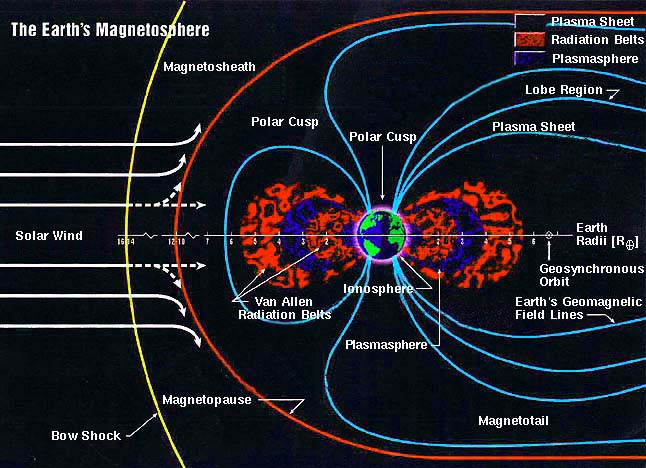
\includegraphics[scale=0.4]{images/earth.jpg}
%%   \caption{Timing Distribution of different Architectures}
%\label{fig:tv}
%\end{figure}
%
%\end{frame}















%%%%%%%%%%%%%
\begin{frame}{Table of Contents}
  \tableofcontents
  %\note{here i want to write something}
  %\pnote{here i want to write something}
\end{frame}

%%%%%%%%%%%%%%%%%%%%%%%%%%%%%%%%%%%%%%%%%%%%%%%%
\section{Introduction}
%%%%%%%%%%%%
%\subsection{\semitransp[-0]{Context}}
\begin{frame}{Context}
%\vspace{-0.9cm}

\begin{block}{Electromagnetic Platform for lightweight Integration/Installation of electrical system in Composite Electrical Aircraft - EPICEA}
\end{block}
\begin{itemize}
\item Avionics engineering issues, reduction of energy, EM issues, CEA.
\item Study the CR effects on aircraft electrical system based on reconfigurable fabric, e.g., FPGAs.
\item Extraction of the faulty response (Signature) --- Sequential Circuits.

\end{itemize}


\begin{block}{Algorithms and methodology for cosmic radiation effects study on aircrafts}
\end{block}
\begin{itemize}
\item Model and analyze the faulty behavior of the sequential circuits.
\item Develop High-Level fault model. 

\end{itemize}




\end{frame}
%%%%%%%%%%%%
%\subsection{\semitransp[40]{Problem Statement}}
\begin{frame}{Problem Statement}
\vspace{-1.5cm}
\begin{block}{Higher Altitude}

\end{block}
\begin{itemize}
\item Vulnerability of the circuits is due to neutrons at an altitude of  50,000 ft~\citep{xilinnseu}.
\item Soft error occur due to radiation ---  radiation event causes enough charge disturbance.
\item Fault caused by Single event upsets (SEUs) --- implications on the behavior of the system.
\item Corrupt the underlying functionality of the hardware.


\item Fault management strategies.
\item High-level fault model for FPGA based circuit.




\end{itemize}




\end{frame}
%%%%%%%%%%%%
%\subsection{\semitransp[40]{Research Objectives}}
\begin{frame}{Research Objectives}

\begin{block}{Analysis and methodology for modelling the faulty sequential circuits}
\end{block}
\begin{itemize}

\item The main objective of this thesis --- is to develop a methodology for modeling the faulty sequential circuits to model the output of the soft error problem at a behavioral level. 
\vspace{0.25cm}
\setbeamertemplate{itemize items}[square]
\begin{itemize}
\item \textbf{Construct} a high-level model from the faulty response observed at a low-level circuit fault emulation.
\vspace{0.25cm}
\item \textbf{Develop} new models that can accurately used to estimate the severity of the faulty behavior from the signature. 



 \vspace{0.25cm}
 \item \textbf{Analyze} the fault origination and propagation for faulty sequential circuits.

\end{itemize}

\end{itemize}




\end{frame}







%\subsection{\semitransp[40]{Research Objectives}}
\begin{frame}{Research Objectives}




%\vspace{0.2cm}

\begin{block}{Faulty behavior model at a high-level of abstraction}
\end{block}

\begin{itemize}

\item{The objective of this thesis is to develop a faulty behavior model
at a high-level of abstraction.} 
\vspace{0.25cm}
\setbeamertemplate{itemize items}[square]
\begin{itemize}
\item The sub-objective of developing a behavioral fault model of a circuit is to generate a \textbf{library of faulty components} reusable at high-level of abstraction.
\vspace{0.25cm}
\item{Develop a \textbf{library of the faulty behavior model} of the sequential circuit
components comprising a Simulink model and VHDL entity. So, each time designers need to analyze potential faulty behavior of a circuit at a high-level of abstraction, designers can utilize the faulty components from the library}.
\vspace{0.25cm}

\item \textbf{VHDL entity} helps to find the device utilization of the target FPGA and it is independent of the technology.
\end{itemize}
\end{itemize}
\end{frame}


%\subsection{\semitransp[40]{Challenges}}

\begin{frame}{Challenges}

\begin{block}{Challenges}

\end{block}


In order to achieve the above mentioned objectives. The main challenges we foresee are:
\begin{itemize}
\item Make a model at higher-level of abstraction from the data extracted at a lower level that represents the behavioral model of the respective signatures. \textbf{High-level model that can recognize low-level fault models.}
\vspace{0.25cm}
%\item Develop a flow to convert faulty behavioral response of a sequential circuit into respective high-level model.
\item Develop an efficient emulation technique, \textbf{Xilinx new tools}.
\vspace{0.25cm}
\item Develop a relationship between the \textbf{bit-flips} and the \textbf{fault-model}.


\end{itemize}




\end{frame}


%\subsection{\semitransp[40]{Contribution}}

\begin{frame}{Contribution}

\begin{itemize}


 \item To model the output of the soft error problem at a behavioral level, e.g., high level modelling technique Hidden Markov Model.
\vspace{0.25cm}
\item This research thesis proposes a fault behavior model with the modeling techniques, e.g., Markovian-analysis in a novel way (utilize hidden Markov model (HMM) to represent faulty behavior of the sequential circuits).
\vspace{0.25cm}
\item Our model will have the capability of efficiently reproduce the signature.The model is used for the signature analysis of the sequential circuit
\vspace{0.25cm}
\item Developing relationship between the FPGA bits emulation information to the faulty models.




\end{itemize}

\end{frame}

\section{Background and Related Work}

\begin{frame}{Background and Related Work}
\vspace{-2.5cm}
\begin{block}{Fundamental concepts and current research}

\end{block}
\begin{itemize}

\item Radiation Environment.
\item Radiation Effects on SRAM based FPGAs.
\item Fault Emulation.
\item Fault behavioral modelling.
\end{itemize}



\end{frame}



\begin{frame}{Radiation Environment}



\begin{block}{Radiation Sources}

\end{block}
\begin{itemize}

\item Galactic Cosmic rays.
\item Radiation from the sun, i.e., solar wind and solar flares.
\item Earth's magnetic Field, e.g., magnetosphere and radiation belts.
\item Atmospheric shower.
\end{itemize}


\begin{block}{Influence of Radiation}
\end{block}
\begin{itemize}

\item First observation (1992), bit flipped~ \\\citep{taber1995investigation}.
\item Aircraft operation of the flight \\ ~\citep{SWE2016}.


\end{itemize}
\vspace{-3cm}

\begin{figure}[h]
 %\centering
  %\captionsetup{justification=left}    
   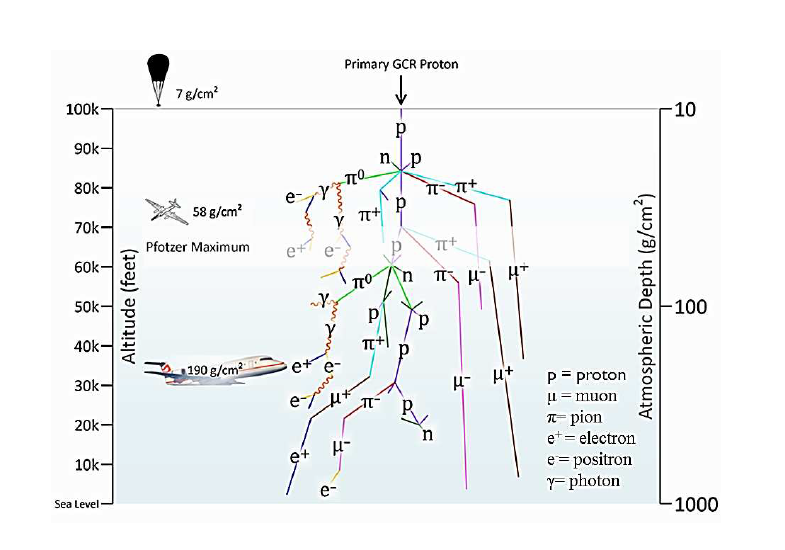
\includegraphics[width=0.37\textwidth, right]{Figures/showerplusaircraft.png}

\label{shower}
\end{figure}
\vspace{-0.7cm} 
\hspace{9.0 cm}



\end{frame}
\begin{frame}{Space Radiation}

\begin{block} {Cosmic Radiation on Aircraft:}

\end{block}

\begin{itemize}
\item \bf{Cosmic rays - high-energy particles that bombard the earth from outer space - are responsilble for the on-flight computer malfunction.

"Something happened in that box that sent the wrong data at various times to the (main) flight computer," ATSB chief commissioner \textit{Martin Dolan} said.}
\end{itemize}

\begin{figure}[]
\centering
%\caption{Timing Variants}
   
  %\input{./images/boxplottpdf}  
  
  %\hspace{-2.8cm} \vspace{4cm}
   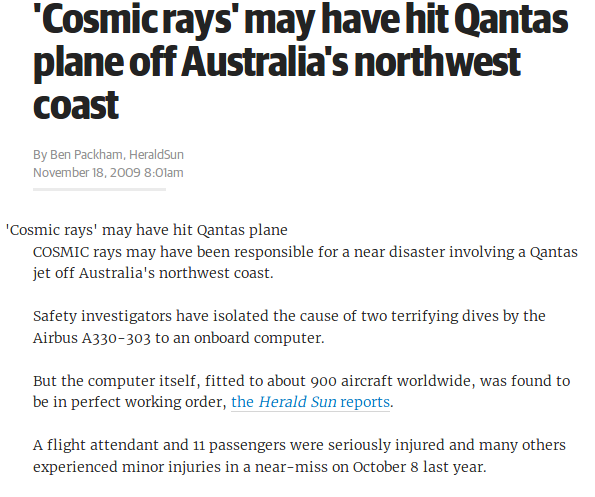
\includegraphics[width=7cm, height=4cm]{images/qantas.png}
%   \caption{Timing Distribution of different Architectures}
\label{fig:tv}
\end{figure}

\end{frame}


\begin{frame}{Radiation Effects on SRAM based FPGAs}

\vspace{-2.0cm}
\begin{block}{Faults caused by cosmic rays in Digital Circuits}

\end{block}
\begin{itemize}

\item Particle strikes a sensitive node in a semiconductor device.
\item Data corruption, transient disturbance.

\item Single Event Effects, e,g., SEU.

\item Soft error and Hard error.

\end{itemize}










\end{frame}





\begin{frame}{Fault Injection}


\vspace{-0.2cm}
\begin{block}{Design Verification by Fault Injection}
\end{block}


\begin{itemize}
\vspace{-0.25cm}
\item \textbf{Simulation}
\vspace{-0.11cm}
\begin{itemize}

\item Simulation based testing is low cost and flexible, but its is difficult to get accurate results.
\item In \citep{violante2004simulation} simulation based testing, during the early design phase when hardware is not ready.
\item \citep{robache2013methodology} demonstrates how signatures allow building high-level models in MATLAB simulink.
\end{itemize}


\item \textbf{Emulation}
\begin{itemize}
\item In \citep{hobeika2014multi} emulation platform for the signature generation, identification of the emulation zone.
\item In \citep{souari2016towards} Fault injection based on the relative sensitivity of the bits. 
\item In \citep{di2014fault} random fault injection.

\end{itemize}



\item \textbf{Radiation Testing}

\begin{itemize}
\item Expensive approach but accurate result.
\item In \citep{hobeika2014multi} effects of radiation on a circuit

\item In \citep{dsilva2015neutron} Flash based FPGA under neutron beam. FIT for FFs, SRAM cell.



\end{itemize}


\end{itemize}





\end{frame}


\begin{frame}{Fault Behavioral Model}
\vspace{-2.0cm}
\begin{block}{Fault Models and Fault Analysis}

\end{block}
\begin{itemize}
\item Behavioral Domain.

\item Transformation Domain.

\item Circuit Domain.
\end{itemize}







\end{frame}


\begin{frame}{Fault Behavioral Model}

\begin{block}{Behavioral  Domain}
\end{block}
\begin{itemize}
\item Emulation using micro-controller. Model based fault injection~\citep{Svenningsson2010}.
\begin{itemize}
\item In \textbf{MY THESIS}: Fault emulation is based on the FPGA, independent of the technology, same VHDL could be ported to different FPGAs.

\end{itemize}

\item In \citep{hayne1999behavioral} Behavioral Fault Mapper. Fault free design and N-faults.  Introduced different fault models, e.g., Dead process.

\begin{itemize}
\item VHDL simulator, no hardware real-time fault emulation, code modification.

\item In \textbf{MY THESIS}: Investigate further their fault models.
\end{itemize}

\item In~\citep{chen2017fault} fault propagation between subsystems.

\begin{itemize}

\item Inconsistency "claim" and "results".

\item System's behavior "Pass" and "Fail".

\item In \textbf{MY THESIS}: Signature into their respective FSM.

\end{itemize} 
\end{itemize}







\end{frame}



\begin{frame}{Fault Behavioral Model}

\begin{block}{Behavioral  Domain}
\end{block}
\begin{itemize}
\item In \citep{mirzadeh2014modeling} fault behavior model developed with a neural network.  
\begin{itemize}
\item Simulation work, no hardware experimental results.
\item Claim to make a library of faulty components.
\item In \textbf{MY THESIS}: provide the library of faulty components.

\end{itemize}



\item In \citep{janschek2017errorsim} Developed tool to simulate different fault models, e.g., offset, stuck-at-fault, etc.



\begin{itemize}


\item Simulation based high-level fault model.
\item Error Propagation Analysis.


\item In \textbf{MY THESIS}: The fault emulation system we describe in this thesis based on the \textbf{real-time bit flip information}. 
\end{itemize} 
\end{itemize}







\end{frame}

\begin{frame}{Fault Behavioral Domain}

\begin{block}{Behavioral Domain}

\end{block}
\begin{itemize}

\item In \citep{hobeika2013flight} New fault models, adaptive control system. But these fault models were also presented in \citep{MOGENTES}.

\item Fault emulation bit information.
\begin{itemize}

\item Xilinx software tool flow \textbf{out-dated}.

\item In \textbf{MY THESIS}: New vivado tools to perform efficient fault emulation.
\end{itemize}


\item In \citep{thibeault2013library} based on the C/C++ description of the application.

\begin{itemize}


\item Technique to convert the circuit into control and data flow graph file.
\item Resource estimation tool to find the resources required to implement an application on an FPGA.
\item The work is based on the \textit{.xdl and .ncd} file \textbf{out-dated}. 
\end{itemize}

\item In \textbf{MY THESIS}: we propose to find the faulty FSM and it's respective VHDL entity to compute resource utilization.

\end{itemize}
 






\end{frame}


\begin{frame}{Fault Behavioral Model}

\begin{block}{Transformation Domain}
\end{block}
\begin{itemize}


\item Transformation of the circuit into respective domain, e,g., BDD \citep{ubar2014modeling}.



\item Boolean Satisfiability Problem (SAT) solvers \citep{shazli2011high}.

\item Mathematical and analytical expressions, fault assumption, assume fault will create an erroneous output.
\end{itemize}
\begin{itemize}
\item \textbf{MY THESIS}: has separated itself from the transformation and work solely on low-level for fault emulation and high-level for behavioral modelling.
\end{itemize} 






\end{frame}




\begin{frame}{Fault Behavioral Model}

\begin{block}{Circuit Domain}

\end{block}
\begin{itemize}
\item The work done in this domain \citep{miskov2007soft}, \citep{miskov2006mars}
 SEUs convergence meaning after how many clock cycles the circuit becomes fault free.
\item Insert the fault into the simulator and observe the output. 


\item Estimate the likelihood of the SET in a sequential circuit, and find the how many clock cycles need to get the SER below the threshold level.
\item Keener to find the part of circuit that has the highest error generating probability.

\begin{itemize}

\item Bottleneck to work in this domain fault assumption, glitch size, assign the probabilities for fault propagation.

\item \textbf{MY THESIS}: will have the real output error probabilities.
\end{itemize}

\end{itemize}






\end{frame}



\section{Proposed Approach}
\begin{frame}{Proposed Approach}



\begin{block}{Relation to State-of-the-Art}
\end{block}
\begin{itemize}
\item \textbf{In literature:} studied fault behavior at high-level/low-level abstraction under the assumption of fault occurrence.
\item \textbf{\cite{robache2013methodology} \cite{hobeika2014multi}}.
\item Fault models for sequential circuit.
\item Fault models in the literature didn't provide any experimental data that these models exist under the radiation or fault emulation.
\item Relationship between these fault models with the underlying hardware architecture regarding bit-flips.

\item Solve with HMM.


\end{itemize}
\vspace{-0.5cm}
\begin{figure}[tb!]
 \centering
  \captionsetup{justification=centering}    
   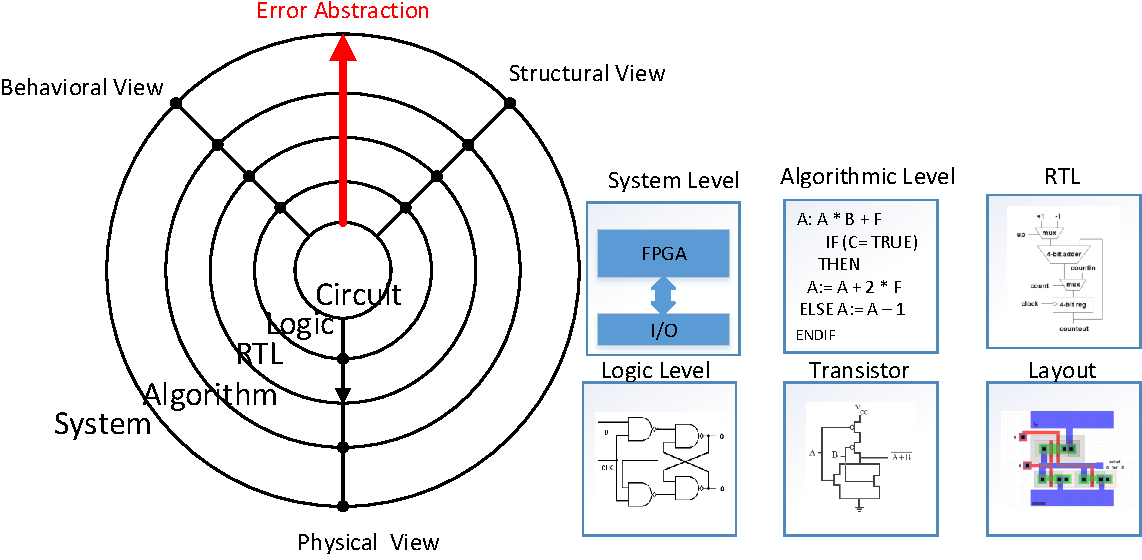
\includegraphics[width=0.3\textwidth]{Figures/ychart-block.pdf}
   \caption{Contribution of this work on Gajski-Kuhn chart.}
\label{fig:ychart}
\end{figure}


\end{frame}



\begin{frame}{Proposed Approach}


\begin{block}{Fault Behavior}
\end{block}

\begin{itemize}

\item Lost Signal or event fault.
\item Stuck Signal.
\item Variable change fault.

\item Changing the specified range of output.
\item Delayed fault, invert fault.
\item Short and open circuit fault. 
\item Stuck-then, Else, Dead Process.

\item Micro-operation fault.
\item Swap Value Fault, Constant fault, amplification.
\item Increase and Decrease.
\end{itemize}


\end{frame}










\begin{frame}{Proposed Approach}

\vspace{-0.2cm}
\begin{block}{Hidden Markov Model}
\end{block}
\begin{itemize}
\item The low-level faulty response to the high-level behavioral model.
\item HMM, which uses the concept of hidden states (stuck-at-fault, delay fault) and observed states (signatures) to find not only the hidden states of the faulty system but also accurately model the observed states.


\end{itemize}

\begin{block}{Why HMM ?}
\end{block}
\begin{itemize}
\item Boolean decision diagram and Algebraic decision diagram.

\item Boolean Satisfiability Problem (SAT).

\item Monte-Carlo Sampling, approximate approach, symbolic method, simulation.

\item \textbf{Need to transform the circuit into their respective tool.}

\item HMM can directly model the system just looking into the signature values.

\item HMM suitable for the systems to model which consists of different observable state (signatures) on different hidden conditions, i.e., fault behavior, e.g., stuck-at-fault, or delay fault.
\end{itemize}


\end{frame}














\begin{frame}{Modelling Hidden Markov Model}

\begin{block}{HMM-Example}

\end{block}

\begin{itemize}

\item To apply the HMM we need a system that generates the probabilistic output pattern, e.g., faulty response of a 3-bit counter.

\item The observed sequence is the "signature" and the hidden is the "stuck-at-fault" or any other fault.




\end{itemize}





\begin{figure}[tb!]
 \centering
  \captionsetup{justification=centering}    
   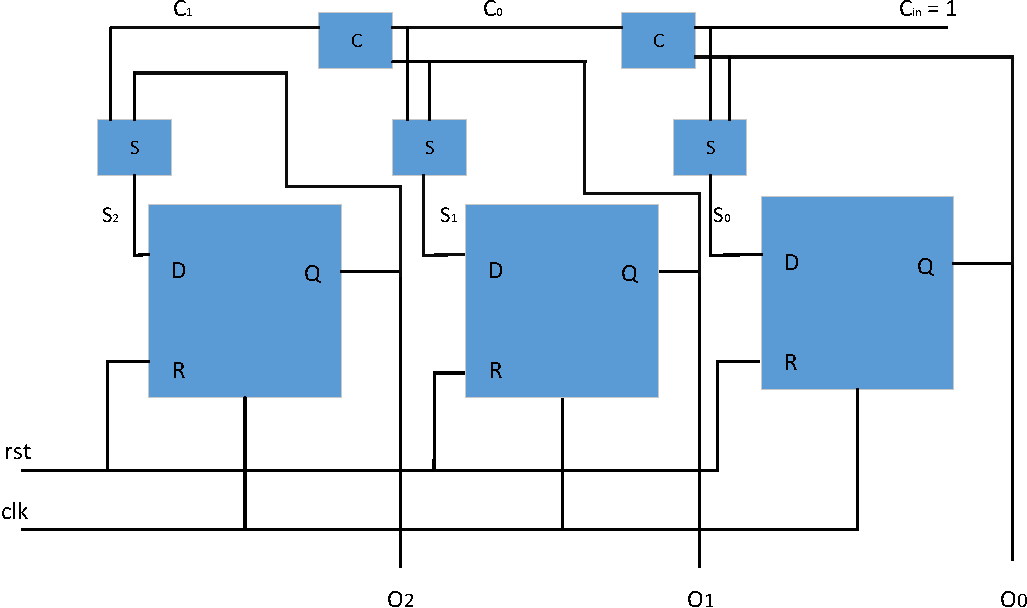
\includegraphics[scale=0.3]{Figures/counter.pdf}
   \caption{3-bit Counter Signature Generation.}
\label{fig:counter}
\end{figure}
\end{frame}

\begin{frame}{Modelling Hidden Markov Model}

\begin{block}{HMM-Example}

\end{block}

\begin{itemize}

\item Four different signature \textit{sign-1, sign-2, sign-3, and sign-3}

\item The observed signatures are probabilistically related to the hidden process. 

\item Signatures: Observable; hidden : faults occur due to bit flip.


\end{itemize}




\begin{figure}[tb!]
 \centering
  \captionsetup{justification=centering}    
   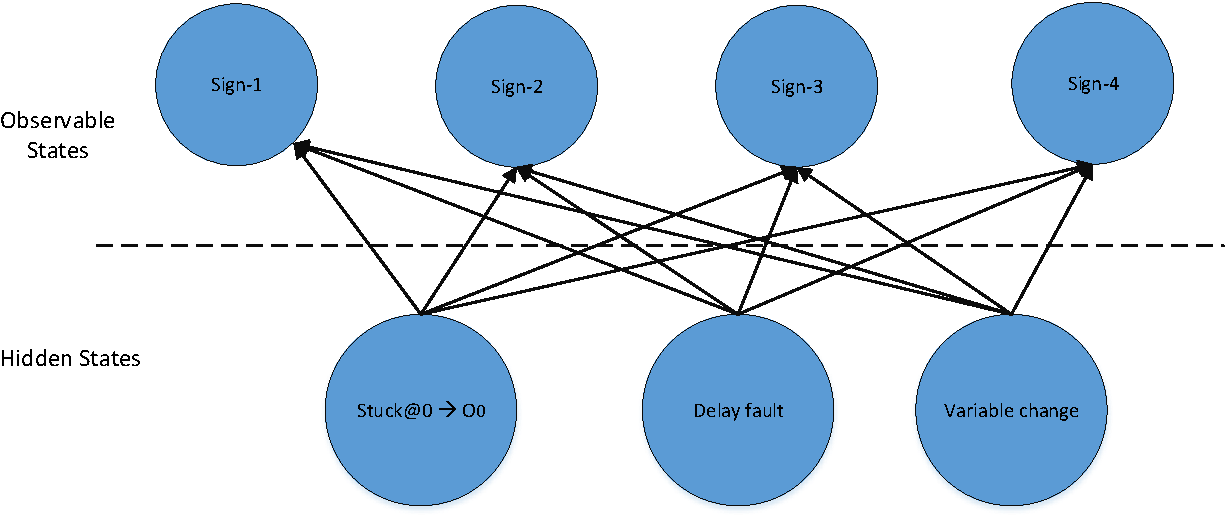
\includegraphics[scale=0.5]{Figures/HMM.pdf}
   \caption{HMM model 3-bit counter.}
\label{fig:HMM-3-bit}
\end{figure}
\end{frame}







\begin{frame}{Modelling Hidden Markov Model}

\begin{block}{HMM applied to the FPGA based emulation system}

\end{block}

\begin{itemize}

\item Outputs are emitted by the system.
\item Observable --- signatures.
\item Bits associated with the fault behavior of the system.
\item HMM seeks to recover the the states from the observed data.



\end{itemize}




\begin{figure}[tb!]
 \centering
  \captionsetup{justification=centering}    
   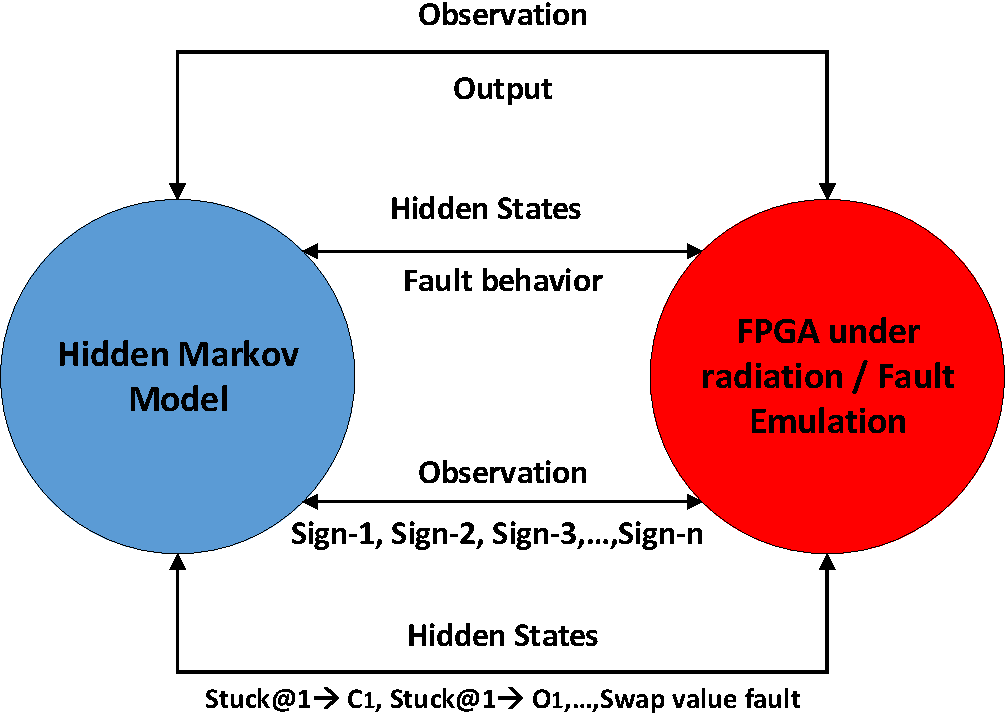
\includegraphics[scale=0.33]{Figures/HMM-air.pdf}
   \caption{Hidden Markov Model to the FPGA based fault emulation system.}
\label{fig:HMM-air}
\end{figure}
\end{frame}
















\begin{frame}{HMM Application for Signature}

\begin{itemize}
\item Compute the probability of a given sequence of signatures.
\item Compute the most probable sequence of states.
\item Given a sequence of observation and learn the best HMM model.

\end{itemize}

\begin{block}{Probability Evaluation}
\end{block}
Find the of an observed signature given an HMM.




\begin{block}{Decoding}
\end{block}
Find the hidden states (fault models) that most probably generated an observed sequence.



\begin{block}{Learning}

\end{block}
Generate an optimized HMM given a sequence of signatures (observations).



\end{frame}






\begin{frame}{HMM Application for Signature}

\begin{block}{Probability Evaluation}
\end{block}
\begin{itemize}


\item For probability evaluation, we need to compute the likelihood of an observed signature sequence $O = {O_1, O_2,...,O_t}$ given a particular HMM $ \Pi = {\pi, A, B}$. The computation of this probability involves all the possible hidden state sequence and evaluate the corresponding probability. 


\item This problem can be solved by using the Forward Algorithm.

\item  This algorithm helps to find the probability of an observe sequence.
\end{itemize}

\end{frame}



\begin{frame}{HMM Application for Signature}

\begin{block}{Decoding Application}
\end{block}
\begin{itemize}
\item The decoding capability of HMM helps to find the sequence of the fault behavior.
\item Viterbi algorithm: Most likely sequence.
\item Posterior decoding: Most likely state each position.
\item Sequence of the hidden states (use in simulator to reproduce the signatures) that give the respective signatures.

\end{itemize}


\begin{figure}[tb!]
 \centering
  \captionsetup{justification=centering}    
   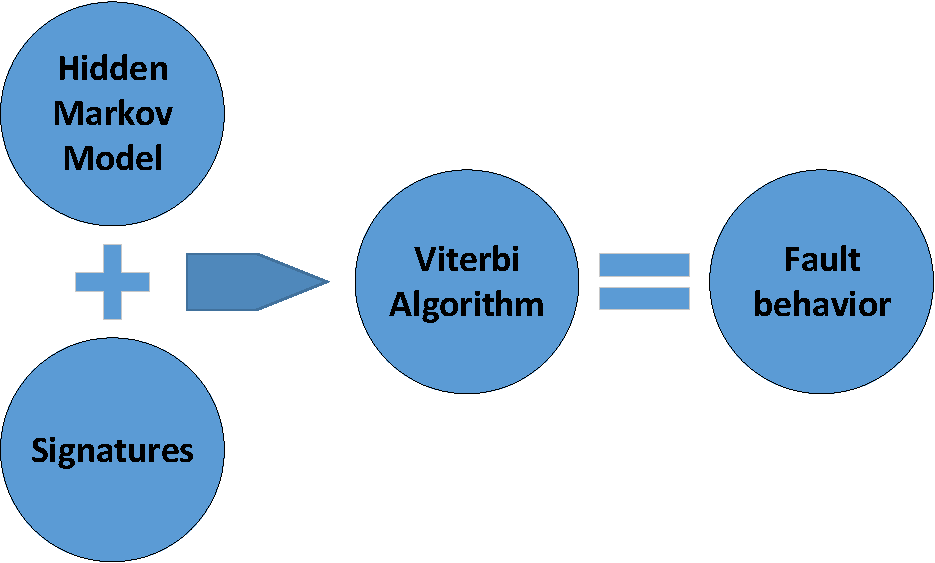
\includegraphics[scale=0.3]{Figures/HMM-plus-viterbi.pdf}
   \caption{Signatures to Fault model.}
\label{fig:HMMsig-Vit}
\end{figure}

\end{frame}



\begin{frame}{HMM Application for Signature}
%\vspace{-1.6cm}
\begin{block}{Learning Application}
\end{block}
\begin{itemize}

\item Optimizing the parameters of the model.

\item Supervised learning: mapping function,  Unsupervised learning: 

\item Model parameters and the observations to find the model that fits the data. 

\item There are three different techniques to do: a) Maximum Likelihood Estimation, b) Viterbi Training, and c) Baum  Welch = Forward-Backward Algorithm.

\item The Viterbi algorithm only finds the single most likely path, and its corresponding probability. Viterbi algorithm only computes an approximation.
\item The Baum-Welch algorithm computes more than this: it does not consider just one path but all possible paths; compute the most likely hidden transition probabilities as well as most likely set of emission probabilities.

\item  Baum-Welch is more accurate and it would therefore lead to better estimates of the model's parameters

 


\end{itemize}
\end{frame}
\begin{frame}{Library Utilization}

\begin{block}{Library of Faulty Components}
\end{block}
\begin{itemize}
\item HMM parameters, probabilities, fault models, hidden states.
\item Library of faulty components.
\item Designers can use to observe the faulty behavior of each sub circuit of the system.

\end{itemize}



\begin{figure}[tb!]
 \centering
  \captionsetup{justification=centering}    
   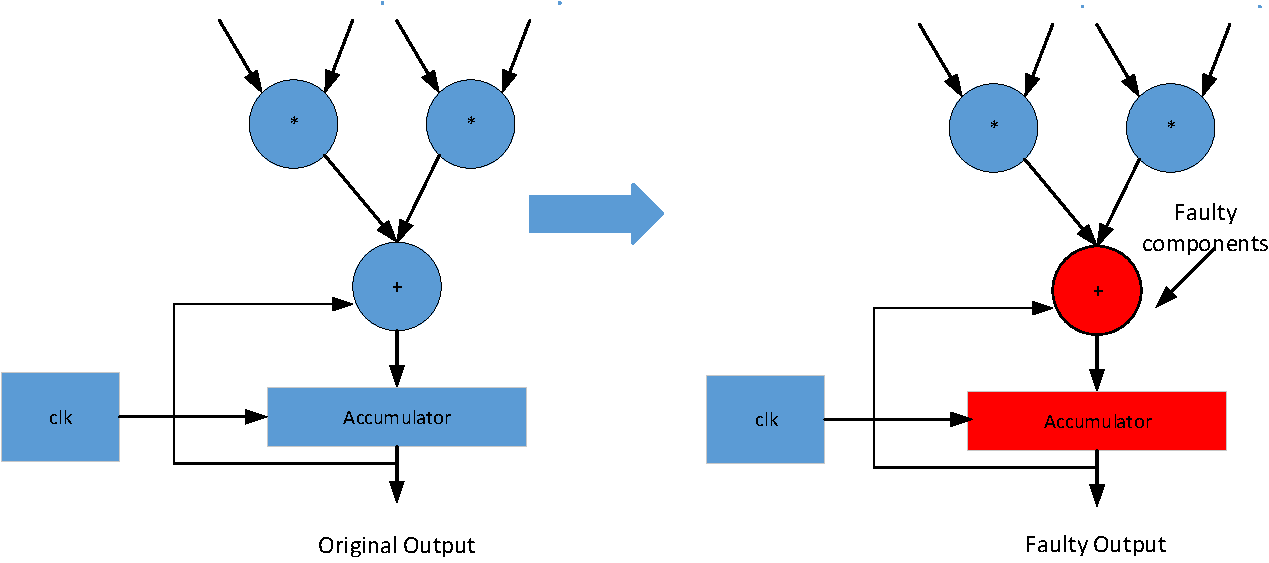
\includegraphics[width=0.6\textwidth, center]{Figures/MAC.pdf}
   %\caption{Example of the faulty Component.}
\label{fig:lib1}
\end{figure}


\end{frame}



\begin{frame}{Library Utilization}

\begin{block}{System's behavior}

\end{block}

\begin{itemize}

\item Create a faulty finite state machine.
\item N-faulty behavioral models.
\item Faulty VHDL entities.

\item Fault occurrences and \\ propagation.
\item Study hardware faults  \\ at high-level of abstraction.
%\item Relationship between the bit-flip information to the fault model.

\vspace{-3.2cm}
\end{itemize}
\begin{figure}[tb!]
 \centering
  \captionsetup{justification=centering}    
   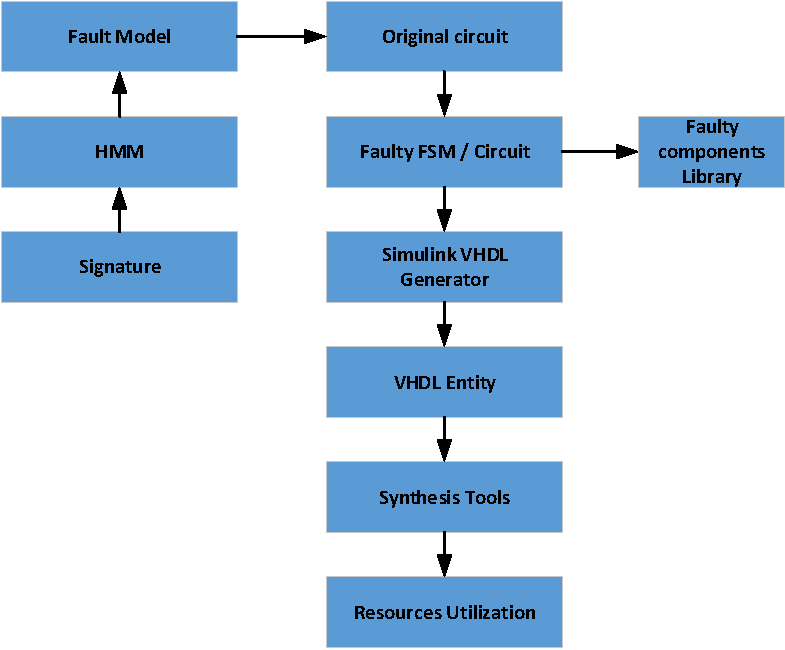
\includegraphics[width=0.55\textwidth, right]{Figures/library.pdf}
   %\caption{VHDL entity creation and usage.}
\label{fig:library1}
\end{figure}


\end{frame}





\begin{frame}{Project Plan}



\begin{block}{Phase: 01}
\end{block}
The emulation platform will be the starting point of the research. We will use the \textbf{sensitivity aware bit-flip} technique for the configuration memory upsets. Selection of a suitable benchmark, which is probably ITC'99 used for the testing purpose and signature generation.





\begin{block}{Phase: 02}

\end{block}
Evaluate the emulation and radiation-based experimental results for signature.


\begin{block}{Phase: 03}
\end{block}
Implement the above-mentioned methodology and high-level model for soft-error of the sequential circuits, i.e., HMM, Faulty FSM, VHDL entities.





\end{frame}






\section{Preliminary Results}
%\subsection{\semitransp[40]{A new Emulation technique based on Bits relative sensitivity}}
\vspace{-2cm}
\begin{frame} {Preliminary Results}

\begin{block}{A new Emulation technique based on Bits relative sensitivity}
\end{block}

\begin{itemize}
\item  The purpose of this work is to studying the relative sensitivity ratio difference between the configuration bit set to "1" and those set to "0" to produce the highly \textbf{accurate behavior} as expected in the real-time radiation testing environment.

\item Prior work: bits at "1" are more likely to generate faults than the bits set at "0"~\citep{souari2016towards}.

\item{In this work, we propose a fault injection method by using relative sensitivity values between the \textbf{bits features}: e.g., bits belong to LUT at "0", bits belong to LUT at "1", bits belong to Non-LUT at "0", bits belong to Non-LUT at "1"}.


\item Signature computed by this method: 2.13 \% percent difference to the adder, and 0.5 \% percent difference to the multiplier circuit observed from the radiation based experiment.




\end{itemize}
\end{frame}




\begin{frame}{Preliminary Results}

\begin{block}{Methodology}
\end{block}
\begin{itemize}

\item Experimental Setup~\citep{hobeika2014multi}.
\item Identification of the bits.
\item Tools have been developed that extract the bit address and the bit location from the \textit{.rbd} file.

\end{itemize}


\begin{figure}[tb!]
 \centering
  \captionsetup{justification=centering}    
   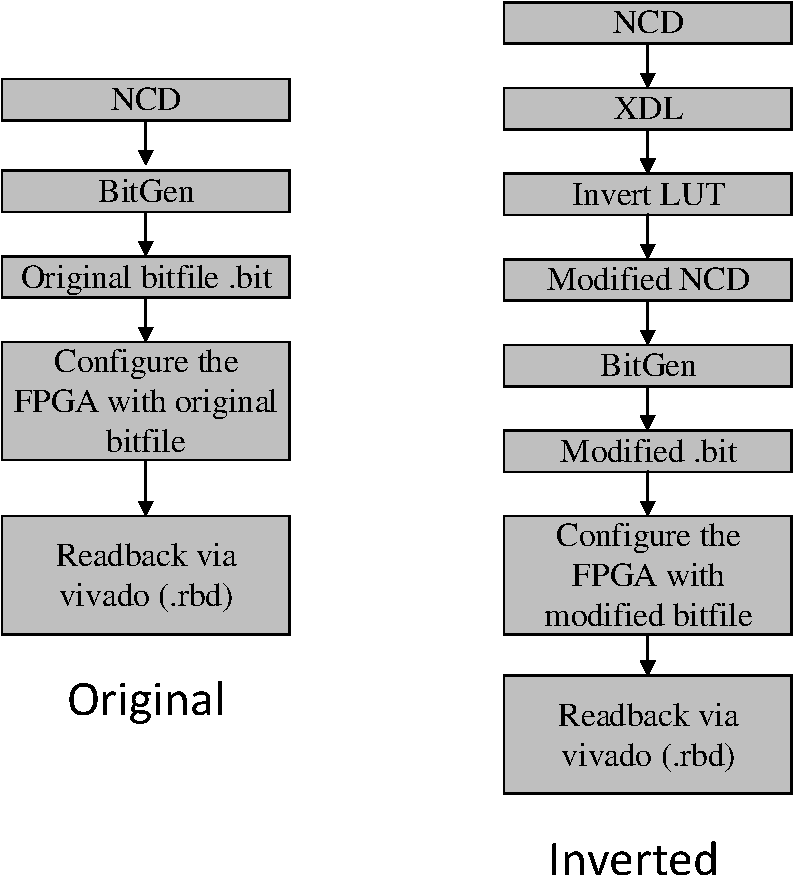
\includegraphics[scale=0.3]{Figures/original-inverted-rbd.pdf}
 
\end{figure}
 %\hspace{9.5cm}Procedure to extract the original .rbd file.




\end{frame}



\begin{frame}{Preliminary Results}

\begin{block}{Bits Classification Algorithm}
\end{block}




\begin{figure}[tb!]
 \centering
  \captionsetup{justification=centering}    
   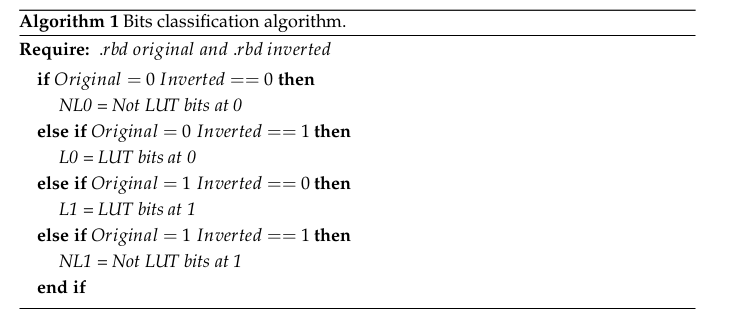
\includegraphics[scale=0.5]{Figures/algo-1.png}
   
\end{figure}






\end{frame}



%%%%%%%%%%%%
%\subsection{\semitransp[40]{DXB-NZAA}}


\begin{frame}{Experimental Results}

\begin{block}{Experimental Results}


\end{block}
\begin{itemize}
\item Emulation performed by flipping the bits at "1" and at "0."
\item Fifty different runs.
\item Percentage of zero Signature.

\end{itemize}
\begin{table}[tb!]
\center
\caption{Adder Emulation Tests Comparison.}
\label{AE}
\begin{tabular}{|c | c| c | c| c| c |} 
 \hline
Test & Zero Signature (\%) & Difference with Radiation (\%)   \\ 
\hline
 
 
 Flip@1& 49.0 &22.5   \\
 \hline
 Flip@0 & 62.8 & 2.2 \\ 
 \hline
 
 Random & 58.1 & 5.5  \\
 \hline
 SA-01 & 56.7 & 7.95\\
 \hline
 SA-02 & 60.1 & 2.13 \\
 \hline
 Radiation & 61.4 & 0  \\
 \hline
 
 
\end{tabular}
\end{table}



\end{frame}




\begin{frame}{Experimental Results}

\begin{block}{Experimental Results}
\end{block}
\begin{table}[tb!]
\center
\caption{Multiplier Emulation Tests Comparison.}
\label{ME}
\begin{tabular}{|c | c| c | c| c| c |} 
 \hline
Test & Zero Signature (\%) & Difference with Radiation (\%)   \\ 
\hline
 
 
 Flip@1& 62.0 &18.3   \\
 \hline
 Flip@0 & 76.0 & 1.9 \\ 
 \hline
 
 Random & 72.1 & 3.3  \\
 \hline
 SA-01 & 73.4 & 1.5 \\
 \hline
 SA-02 & 74.9 &  0.5\\
 \hline
 Radiation & 74.6 & 0  \\
 \hline
 
 
\end{tabular}
\end{table}



\end{frame}

\begin{frame}{Experimental Results}

\begin{block}{Bit Flip Validation}

\end{block}

\begin{table}[tb!]
\center
\caption{Relative Sensitivity from experimentation performed at TRIUMF.}
\label{RS}
\begin{tabular}{|c | c| c | c | } 
 \hline
Bits feature & \makecell*{Relative Sensitivity}  & \makecell*{Adder \\(Observed)} & \makecell*{Multiplier \\ (Observed)}  \\ 
%\hline
%& \multicolumn{1}{c}{ (Theoretical)} \\
%& & \multicolumn{1}{c}{observed} \\
 \hline
 
 Bits@0 non LUT & 1.00 & 1.00 & 1.00 \\
 \hline
 Bits@1 non LUT& 1.41  & 1.43&1.44\\ 
 \hline
 
 Bits@0 LUT & 2.06 &2.08 &2.09\\
 \hline
 Bits@1 LUT & 1.91 &1.92&1.91\\
 \hline
% \hline
 
 
\end{tabular}
\end{table}










\end{frame}








%\subsection{\semitransp[40]{Signature for High-level Modelling}}
\begin{frame}{Signature for High-level Modelling}
\vspace{-1.0cm}
\begin{block}{Signature for High-level Modelling}
\end{block}
\begin{itemize}

\item Signature Observed at the Triumf Experiment~\citep{hobeika2014multi}.
\item Signature Observed FPGA Emulation.
\item High-level Model\footnote{Prof. Claude performed experiments on tessent.}.
\item Adder signature fault model.
\item Multiplier signature fault model.
\end{itemize}

\end{frame}



\begin{frame}{Signature for High-level Modelling}

\begin{block}{Adder signature fault model}
\end{block}
\begin{itemize}
\item Positive signatures can be modeled as single stuck-at-one fault model.

\item The negative signature can be modeled as single as stuck-at-zero fault model.

\end{itemize}


\begin{table}[tb!]
\center
\caption{Adder Signature Format.}
\label{adder signature format}
\begin{tabular}{|c | c |} 
 \hline
Decimal Format & Hexadecimal   \\ 
\hline
 
 
 $16$& $00000010$    \\
 \hline
 $64$ & $00000040$  \\ 
 \hline
 
 $128$ & $00000080$  \\
 \hline
 $-1024$ & $FFFFFC00$ \\
 \hline
 $-512$ & $FFFFFE00$ \\
 \hline
 $-8$ & $FFFFFFF8$   \\
 \hline
 
 
\end{tabular}
\end{table}





\end{frame}



\begin{frame}{Signature for High-level Modelling}

\begin{block}{Adder signature fault model}
\end{block}

\vspace{-0.25 cm}
\textbf{Rule\#01}
\textbf{Example:}

\hrule height 2pt width \hsize \kern 1pt \hrule width \hsize height 1pt

$Original$ $=$ $24$; $binary $ $ equivalent$ $11000$ \\
\hspace{-0.15cm} $Faulty$ $=$ $8$; $binary $ $ equivalent$ $01000$ \\
$fourth$ $bit$ $flipped$ $from$ $"1"$ $to$ $"0"$

$signature$ $=$ $8$ - $24$ $=$ $8$ $+$ $(-24)$ $=$ $16$ \\
$4^{th}$ $ bit $ $flipped$; $i$  $=$ $4$, $2^{4}$ $=$ $16$
\vspace{0.01cm}
\hrule height 2pt width \hsize \kern 1pt \hrule width \hsize height 1pt
%\vspace{0.25 cm}

\textit{\begin{equation}
\label{eq:2}
  \pm2\textsuperscript{i}    \hspace{0.5 cm} 0\leq i \leq15
\end{equation}}


\vspace{-0.5cm}
\textbf{Rule\#02}


\textbf{Example valid signatures (Adder) for rule \# 02:}
\hrule height 2pt width \hsize \kern 1pt \hrule width \hsize height 1pt
\begin{center}
$1010 0000 0000 0000$ \\
$1000 1000 0000 0000$ \\
$1000 1000 0000 0000$ \\
$1000 0000 0000 0100$ \\
$1000 0000 0000 0001$ \\
\end{center}
\hrule height 2pt width \hsize \kern 1pt \hrule width \hsize height 1pt



\end{frame}


\begin{frame}{Signature for High-level Modelling}

\begin{block}{High Level Model of Adder in Simulink}

\end{block}


\begin{figure}[tb!]
 \centering
  \captionsetup{justification=centering}    
   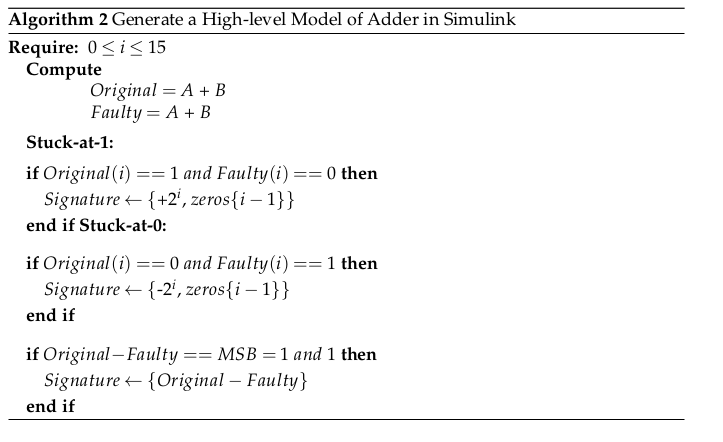
\includegraphics[scale=0.44]{Figures/algo-2.png}
   

\end{figure}



\end{frame}














%\subsection{\semitransp[40]{DXB-YYZ}}
\begin{frame}{Signature for High-level Modelling}

\begin{block}{Multiplier signature fault model}
\end{block}
\begin{itemize}
\item 8-bit multiplier.
\item Two rules have been formulated.

\item \textbf{Rule \# 01:} This rule defines the signature can be expressed by the Equation \ref{eq:2} that represents the stuck-at-1 and stuck-at-0 fault model, and the multiplier behaves as the bit flipped occurred at the output of the multiplier.  \\
\item \textbf{Rule \# 02:} The rule number two defines the format of the signature obtained when a bit flipped cause the multiplier to behave as if when an input bit is either stuck-at-0 or stuck-at-1 can be represented \{$-$$A$ $\times$ $2^{i}$ $or$  $-$$B$ $\times$ $2^{i}$ \}, \{$+$$A$ $\times$ $2^{i}$ $or$  $+$$B$ $\times$ $2^{i}$ \} respectively. 

\end{itemize}

\end{frame}

\begin{frame}{Signature for High-level Modelling}

\begin{block}{High-level model of multiplier in Simulink}
\end{block}



\begin{figure}[tb!]
 \centering
  \captionsetup{justification=centering}    
   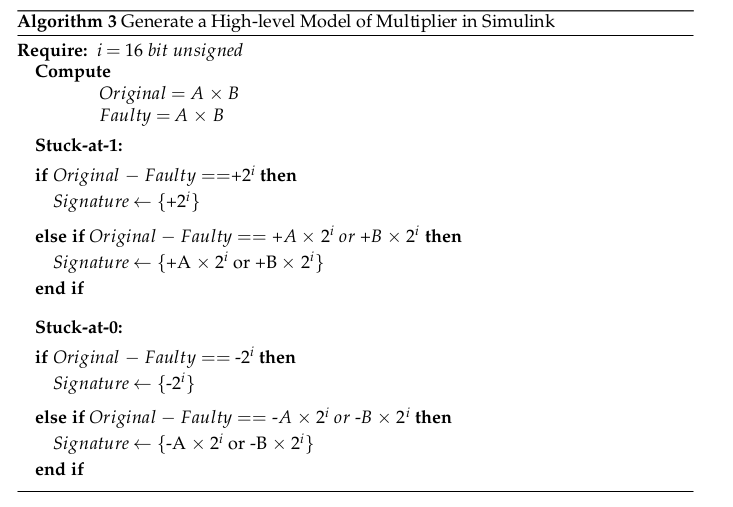
\includegraphics[scale=0.35]{Figures/algo-3.png}
   

\end{figure}



\end{frame}

%\subsection{\semitransp[40]{Signature for Sequential Circuit}}

\begin{frame}{Signature for Sequential Circuit}
\vspace{-3cm}
Derived the Signature for: 

\begin{itemize}

\item 3-bit counter
\item FIR Filter

\end{itemize}

\end{frame}
\begin{frame}{Signature for Sequential Circuit}

\begin{block}{3-bit counter}
\end{block}
\begin{itemize}

\item 3-bit counter in MATLAB Simulink

\item Derived the signatures by stuck-at-fault model. 

\item Stuck-at-1$\rightarrow B_0$.

\end{itemize}



\vspace{-2.0cm}
\begin{figure}[tb!]
 %\centering
  \captionsetup{justification=centering}    
   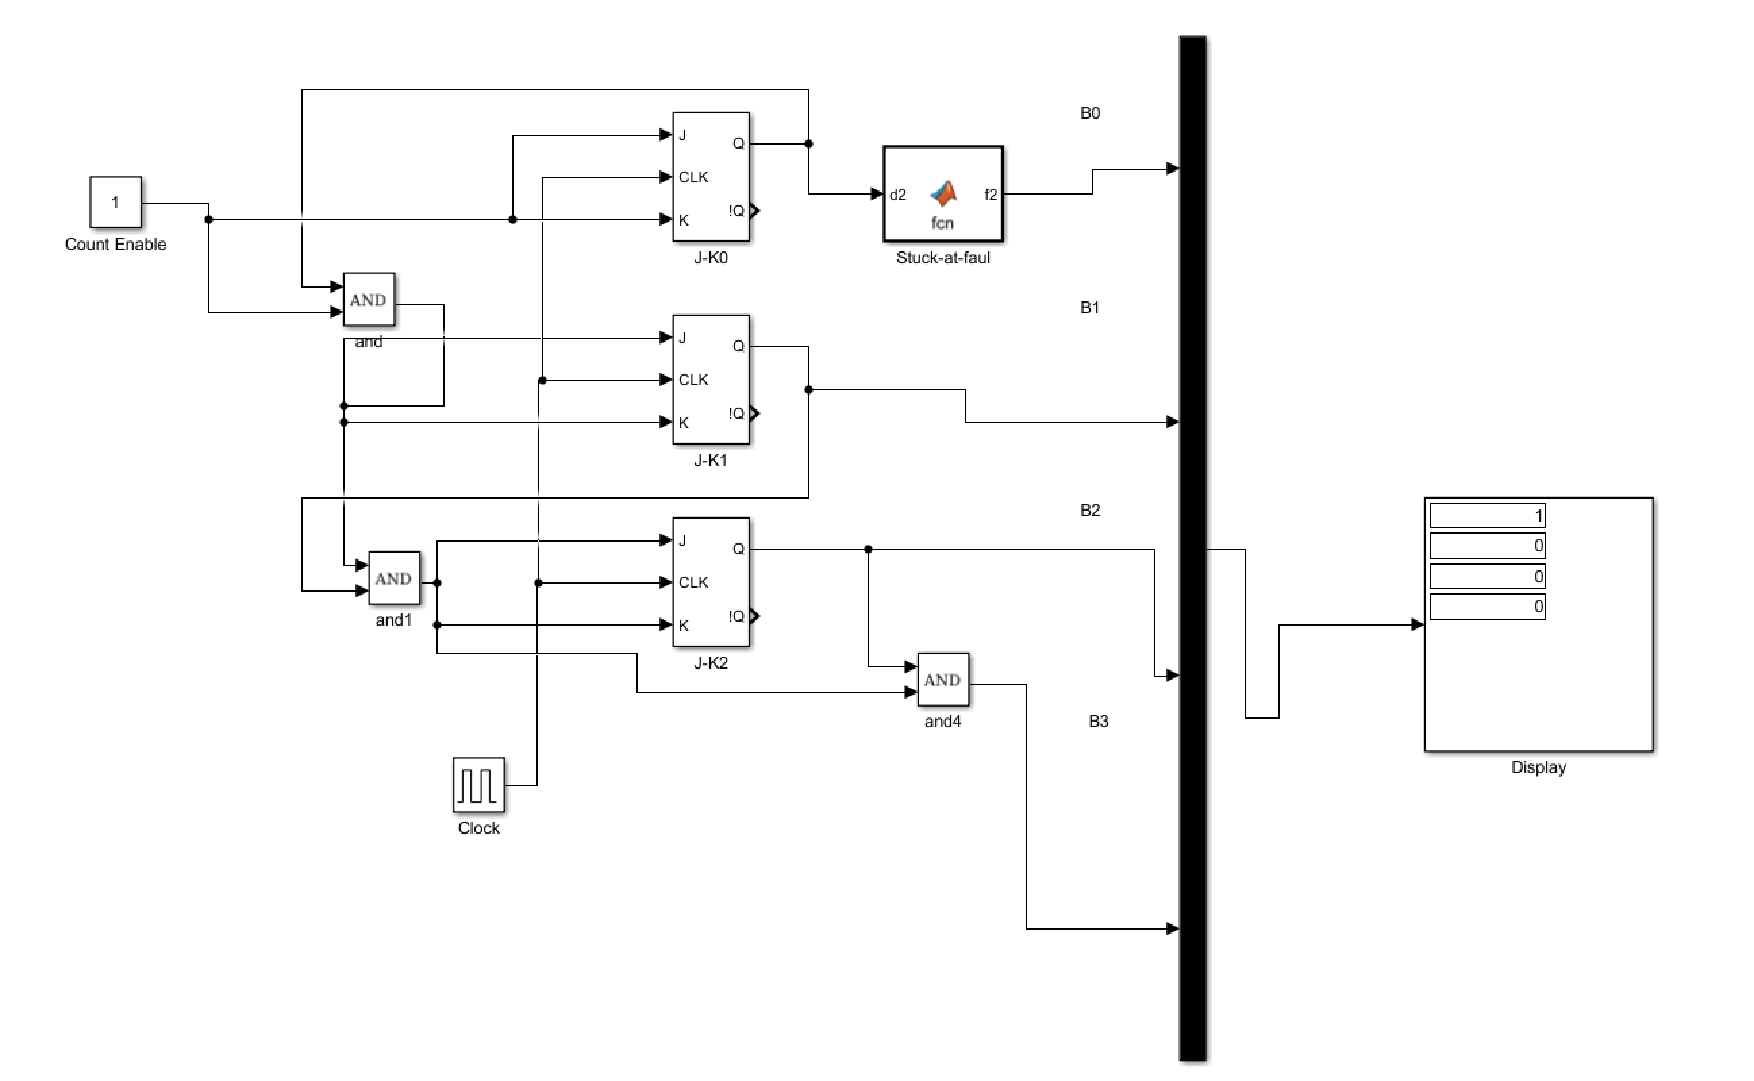
\includegraphics[width=7.5cm, height=5.5cm, right]{Figures/matlab-counter.pdf}
  
\label{fig:matlab}
\end{figure}
\vspace{-5.0cm}
%\vspace{-5.0cm}
\begin{table}[tb!]

%\caption{Stuck-at-1$\rightarrow B_0$.}
\label{stuck}
\scalebox{0.55}{

\hspace{-15.0cm}
\begin{tabular}{|c | c| c | c| } 
 \hline
 \rowcolor{lightgray}
Faulty Value (Binary) & Faulty Value & Original Value & Arithmetic Signature   \\ 
\hline
 
 
 001& 1 &0 & -1  \\
 \hline
 011 & 3 & 1 & -2 \\ 
 \hline
 
 101 & 5 & 2 & -3 \\
 \hline
 111& 7& 3& -4 \\
 \hline
 001 & 1  &  4& 3 \\
 \hline
 011 & 3 & 5 &2  \\
 \hline
 101 & 5 & 6 & 1 \\
 \hline
 111 & 7 & 7 & 0 \\
 \hline
 
 
\end{tabular}
}
\end{table}







\end{frame}

\begin{frame}{Signature for Sequential Circuit}

\begin{block}{FIR filter}
\end{block}
\begin{itemize}
\item Stuck-at-fault model to different nodes in the FIR filter.
\item Stuck-at-0$\rightarrow X_1$.
\end{itemize}


\begin{figure}[tb!]
 \centering
  \captionsetup{justification=centering}    
   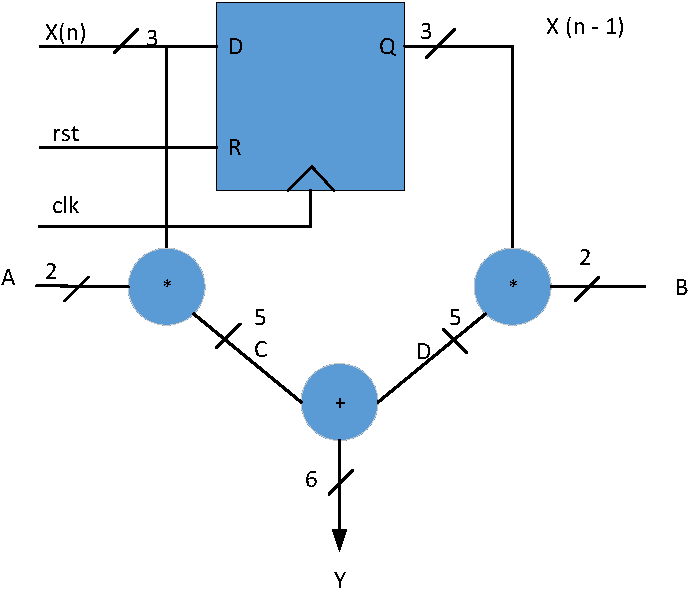
\includegraphics[width=0.4\textwidth, right]{Figures/FIR.pdf}
   
\label{fig:filter}
\end{figure}

\vspace{-6.0cm}

\begin{table}[tb!]
%\center
%\caption{Stuck-at-0$\rightarrow Y_0$.}
\hspace{-6.0cm}
\scalebox{0.55}{
\begin{tabular}{|c | c| c | c| c |} 

 \hline
 \rowcolor{lightgray}
Decimal Golden & Binary & Stuck@0$\rightarrow X_1$ & Decimal Faulty & Arithmetic Signature   \\ 
\hline
 
 
 0 & 000000 & 000 & 0 & 0  \\
 \hline

 1 & 000001 & 001 & 1 & 0 \\
 \hline
 
 6 & 000110 & 000 & 2 & 4 \\
 \hline
 15 & 001111 & 001 & 3 & 12 \\
 \hline
 14 & 001110 & 100 & 10 & 4 \\
 \hline
 27 & 011011 & 101 & 27 & 0 \\
 \hline
 11 & 001011 & 100 & 9 & 2 \\
 \hline
 0 & 000000 & 101 & 0 & 0 \\
 \hline
 0 & 000000 & 100 & 0 & 0 \\
 \hline
 11 & 001011 & 101 & 9 & 2 \\
 \hline
 18 & 010010 & 100 & 18 & 0 \\
 \hline
 
 21 & 010101 & 001 & 15 & 6 \\
 \hline
 10 & 001010 & 000 & 2 & 8 \\
 \hline
 9 & 001001& 001 & 3 & 6 \\
 \hline
 1 & 000001 & 000 & 1 & 0 \\
 \hline
 0 & 000000 & 001 & 0 & 0 \\
 \hline




 
 
\end{tabular}
}
\end{table}


\end{frame}

\section{Time Table}

\begin{frame}{Time Table}
\vspace{-0.5cm}
\begin{block}{Task Development}
\end{block}


\begin{itemize}
\vspace{-0.5cm}
\item \textbf{(1) Conference paper - $2018$:} \\
The new fault emulation strategy,\\bits sensitivity, and it's feature.

\item \textbf{(2) Conference Paper - $2018$:} \\

High-level fault models for \\adder and multiplier.
\item \textbf{(3) Conference Paper - $2019$ :} \\

Fault modelling with HMMs. \\
Signature for sequential circuits. \\ New emulation technique.\\
Fault models.

\vspace{0.35cm}

\item \textbf{Journal Paper - 2019:} \\
Emulation technique, low-level signature generation, Signature comparison, high-level modelling, faulty FSM, VHDL entity, faulty components library.

\end{itemize}






\vspace{-7.7cm}

\begin{figure}[tb!]
 \centering
  \captionsetup{justification=centering}    
   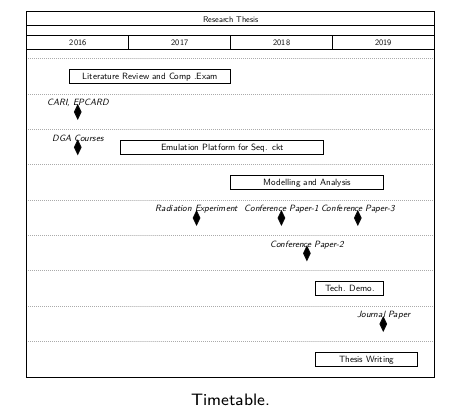
\includegraphics[width=0.49\textwidth, right]{Figures/time-table.png}
   
\label{fig:filter}
\end{figure}





%\begin{center}
%\begin{figure}[h]
%\label{timetable}
%%\centering
%\scalebox{0.40}{
%\begin{tikzpicture}
%\begin{ganttchart}[
%x unit=0.36cm,
%y unit title=1.0cm,
%y unit chart=1.5cm,
%%vgrid,
%hgrid,
%inline,
%]{1}{48}
%\gantttitle{Research Thesis}{48} \\
%\gantttitle{2016}{12} \gantttitle{2017}{12} \gantttitle{2018}{12} \gantttitle{2019}{12}\\
%
%\ganttbar[bar height=.4]{Literature Review and Comp .Exam}{6}{24}\\
%%\ganttbar[bar height=.4]{DGA courses \& CARI, EPCARD}{6}{12}\\
%\ganttmilestone[]{CARI, EPCARD}{6}\\
%\ganttmilestone[]{DGA Courses}{6}
%\ganttbar[bar height=.4]{Emulation Platform for Seq. ckt}{12}{35} \\
%%ganttmilestone[]{Radiation Experiment}{12} \\
%\ganttbar[bar height=.4]{Modelling and Analysis}{25}{42} \\
%\ganttmilestone[]{Radiation Experiment}{20}
%\ganttmilestone[]{Conference Paper-1}{30}
%\ganttmilestone[]{Conference Paper-3}{39}\\
%\ganttmilestone[]{Conference Paper-2}{33}\\
%%\ganttbar[bar height=.4]{Novel Timing analysis techniques}{22}{38} \\
%%\ganttmilestone[]{DAC}{36}\\
%%\ganttbar[bar height=.4]{FPGA Implementation}{27}{38} \\
%%\ganttmilestone[]{TRETS}{40}\\
%\ganttbar[bar height=.4]{Tech. Demo.}{35}{42} \\
%\ganttmilestone[]{Journal Paper}{42}\\
%\ganttbar[bar height=.4]{Thesis Writing}{35}{46}
%%\ganttmilestone[]{Thesis}{44}\\
%%\ganttbar[bar height=.4]{The \emph{PolyOrbite} Project}{1}{44} 
%%\ganttlink{elem0}{elem1}
%%\ganttlink{elem0}{elem2}
%%\ganttlink{elem0}{elem3}
%%\ganttlink{elem3}{elem4}
%%\ganttlink{elem5}{elem6}
%%\ganttlink{elem5}{elem7}
%%\ganttlink{elem7}{elem8}
%\end{ganttchart}
%\end{tikzpicture}
%}
%
%\caption{Timetable.}
%\label{timetable}
%\end{figure}

%\end{center}


\end{frame}

%
%\begin{frame}{Time Table}
%
%
%\begin{itemize}
%
%\item \textbf{(1) Conference paper - $2018$:} \\
%In the first conference paper, we will present the new fault emulation strategy based on the bits sensitivity, and it's feature.
%
%\item \textbf{(2) Conference Paper - $2018$:} \\
%
%High-level fault models for adder and multiplier.
%\item \textbf{(3) Conference Paper - $2019$ :} \\
%
%Fault modelling with HMMs. \\
%Signature generation for sequential circuits based on the new emulation technique.
%Fault models.
%
%
%\item \textbf{Journal Paper - 2019:} \\
%Emulation technique, low-level signature generation, Signature comparison, high-level modelling, faulty FSM, VHDL entity, faulty components library.
%
%\end{itemize}
%
%
%
%
%
%
%\end{frame}















\section{}
\begin{frame}
\begin{center}
\Huge Thank You! \\
\Huge Questions and Suggestions
\end{center}

\end{frame}



%%%%%%%%%%%%%%%%%%%%%%%%%%%%%%%%%%%%%%%%%%%%%%%%




%%%%%%%%%%%%%%%%%%%%%%%%%%%%%%%%%%%%%%%%%%%%%%%%%
%\section*{References}
%\begin{frame}[allowframebreaks]
%        \frametitle{References}
%        \bibliographystyle{IEEEtran}
%        \bibliography{polymtl_presentation.bib}
%\end{frame}

\section*{References}
\begin{frame}[allowframebreaks]
        \frametitle{References}
        \bibliographystyle{agsm}
        \bibliography{polymtl_presentation.bib}
\end{frame}




\end{document}